\documentclass{sysupptthesis}

\AddToHook{shipout/foreground}{\BackgroundPicture}
\author{王伊煜}
\title{新时代地外文明搜寻}
\subtitle{本科毕业论文答辩报告}
\institute{中山大学 物理与天文学院}
\date{2026年4月}

\begin{document}

% ============ 封面 ============
\begin{frame}
    \titlepage
    \vspace*{-0.5cm}
    \begin{center}
        {\large\textbf{中山大学}}\\[0.3em]
        {\normalsize 答辩人：王伊煜 \quad|\quad 学号：22344140}\\[0.2em]
        {\normalsize 指导教师：张泳 教授}
    \end{center}
\end{frame}

% ============ 目录 ============
\begin{frame}{目录}
    \tableofcontents[sectionstyle=show,subsectionstyle=show/shaded/hide]
\end{frame}

% ============================================================
\section{研究背景与意义}
% ============================================================

\begin{frame}{研究背景}
    \begin{block}{历史起源}
        \begin{itemize}
            \item 1959年：Cocconi与Morrison在\textit{Nature}发表奠基论文，系统论证星际通信信号可被观测
            \item 1960年：Frank Drake在绿岸天文台实施奥兹玛计划，现代SETI由此开启
            \item 从窄带监听、冷战时期大尺度设想到当代技术特征（technosignature）搜索框架
        \end{itemize}
    \end{block}

    \begin{block}{核心科学困难}
        \begin{itemize}
            \item 搜索空间极大、信号形式高度不确定
            \item 观测覆盖长期不足，零结果难以形成强约束
            \item 涉及极端稀有目标、超大参数空间等前沿方法论问题
            \item SKA的出现为重新理解SETI科学意义提供新切入点
        \end{itemize}
    \end{block}
\end{frame}

\begin{frame}{研究意义与核心问题}
    \defination{核心命题}{
        SETI如何从长期具有争议性的探索议题，逐步转化为更具可检验性的观测科学问题？
    }

    \begin{block}{研究思路}
        \begin{itemize}
            \item 将天区覆盖、频率覆盖和灵敏度视为三个最关键维度
            \item 建立统一观测坐标系，比较不同历史阶段代表性计划
            \item 论证SKA为何可能成为新时代SETI研究的\textbf{设施拐点}
            \item 推动SETI走向以参数空间约束为特征的观测科学
        \end{itemize}
    \end{block}
\end{frame}

% ============================================================
\section{资料来源与三维分析框架}
% ============================================================

\begin{frame}{资料来源与文献基础}
    \begin{block}{四类材料}
        \begin{itemize}
            \item \textbf{ADS文献数据}：1960--2025年SETI文献阶段性变化分析
            \item \textbf{经典文献与综述}：从Cocconi-Morrison到technosignature问题脉络
            \item \textbf{代表性观测论文}：Breakthrough Listen对1327颗近邻恒星1.10--3.45 GHz搜索
            \item \textbf{SKAO官方文档}：系统规格和性能资料
        \end{itemize}
    \end{block}

    \begin{block}{双口径文献集}
        \begin{itemize}
            \item \textbf{严格核心文献集}：标题/摘要含SETI、technosignature等核心词 $\rightarrow$ \textbf{778篇}（天文学同行评议）
            \item \textbf{全量相关文献集}：扩展至天文学与物理学 $\rightarrow$ \textbf{1519篇}（宽口径趋势观察）
            \item 双口径并行，避免宽泛关键词噪声与边界过严的低估
        \end{itemize}
    \end{block}
\end{frame}

\begin{frame}{三维分析框架}
    \begin{block}{1. 天区覆盖——累计被观测的天空面积（deg$^2$）}
        \begin{itemize}
            \item 定点监听：按 $N_{\text{tgt}} \times \Omega_b$（主波束面积）近似
            \item 巡天计划：采用公开面积量级，强调数量级比较
        \end{itemize}
    \end{block}

    \begin{block}{2. 频率覆盖——实际搜索到的频率范围（GHz）}
        \begin{itemize}
            \item $\Delta f = f_{\max} - f_{\min}$：实际搜了多宽，而非设备理论上能看多宽
            \item 区分"设备名义能力"与"计划实际搜索范围"
        \end{itemize}
    \end{block}

    \begin{block}{3. 灵敏度——最小可探测信号能力}
        \begin{itemize}
            \item 严格用 $A_{\text{eff}}/T_{\text{sys}}$、SEFD和辐射计方程
            \item 图表中以集光面积（m$^2$）作直观代理
        \end{itemize}
    \end{block}
\end{frame}

% ============================================================
\section{SETI历史演化分析（1960--2025）}
% ============================================================

\begin{frame}{SETI发展的四个阶段}
    \begin{columns}[T]
        \begin{column}{0.48\textwidth}
            \begin{block}{第一阶段（1960s--70s）：开创期}
                \begin{itemize}\small
                    \item Cocconi-Morrison（1959）；Drake奥兹玛（1960）
                    \item 累计4篇，年均 $\bar{N} \approx 0.36$篇/年
                    \item 窄带监听技术路径确立
                \end{itemize}
            \end{block}
            \begin{block}{第二阶段（1971--92）：扩张期}
                \begin{itemize}\small
                    \item NASA HRMS专项
                    \item 381篇，$\bar{N} \approx 17.3$篇/年
                    \item 增长率 $g = 9425\%$，制度化推进
                \end{itemize}
            \end{block}
        \end{column}
        \begin{column}{0.48\textwidth}
            \begin{block}{第三阶段（1993--2015）：转型期}
                \begin{itemize}\small
                    \item NASA项目终止后的分散化增长
                    \item 563篇，$\bar{N} \approx 24.5$篇/年
                    \item 跨学科持续积累
                \end{itemize}
            \end{block}
            \begin{block}{第四阶段（2016--25）：复兴期}
                \begin{itemize}\small
                    \item BL启动、FAST参与
                    \item 571篇，$\bar{N} \approx 57.1$篇/年
                    \item 年均增幅 $133\%$，明显加速
                \end{itemize}
            \end{block}
        \end{column}
    \end{columns}
\end{frame}

\begin{frame}{四阶段示意图}
    \begin{center}
        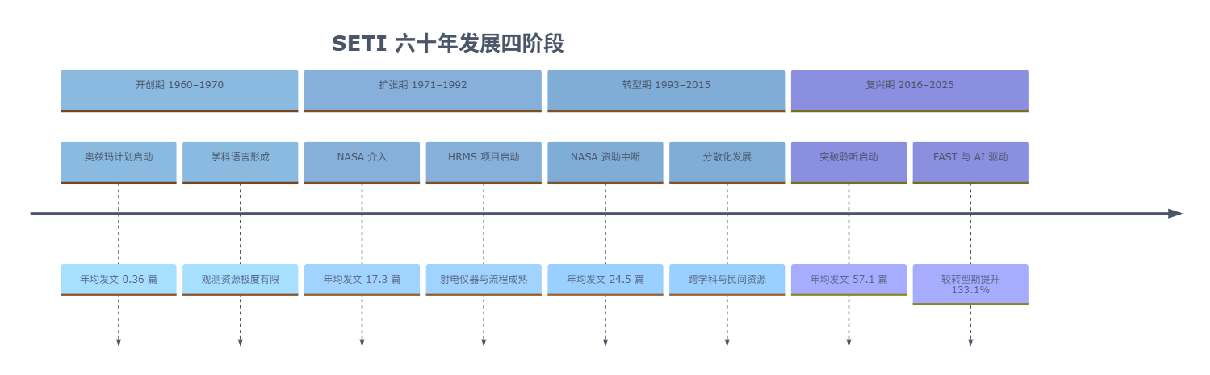
\includegraphics[width=0.75\textwidth]{fig/fig_01_p20.png}
    \end{center}
    \vspace{-0.3em}
    \begin{center}\small
        图3.1 SETI六十年发展四阶段示意图
    \end{center}
\end{frame}

\begin{frame}{文献统计：严格核心集与全量集}
    \begin{columns}[T]
        \begin{column}{0.48\textwidth}
            \begin{center}
                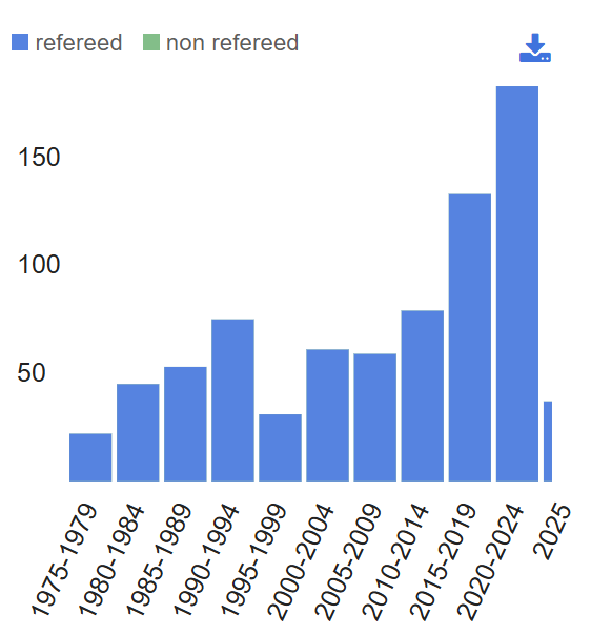
\includegraphics[width=\textwidth]{fig/fig_02_p21.png}\\[0.3em]
                {\small 严格核心文献集（778篇）}
            \end{center}
        \end{column}
        \begin{column}{0.48\textwidth}
            \begin{center}
                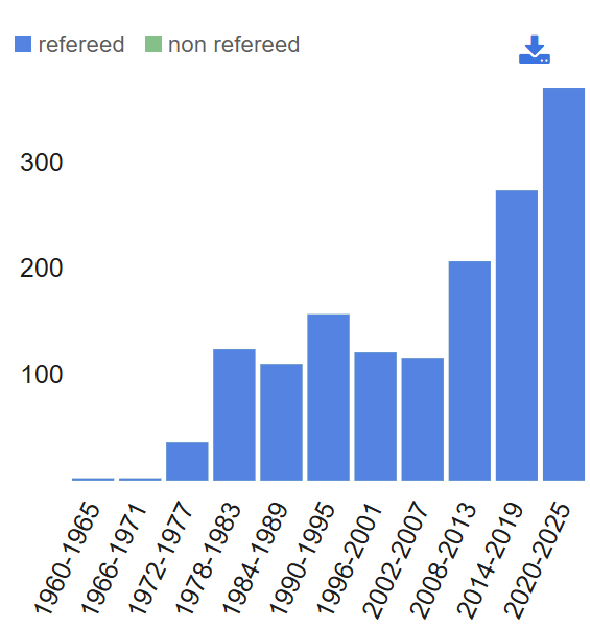
\includegraphics[width=\textwidth]{fig/fig_03_p21.png}\\[0.3em]
                {\small 全量相关文献集（1519篇）}
            \end{center}
        \end{column}
    \end{columns}
    \vspace{0.5em}
    \begin{block}{核心发现}
        SETI领域的兴衰更主要受\textbf{设备能力、资助结构及相关学科发展条件}影响，而非单纯取决于是否发现可信信号。
    \end{block}
\end{frame}

\begin{frame}{核心引用与阅读数据}
    \begin{columns}[T]
        \begin{column}{0.48\textwidth}
            \begin{center}
                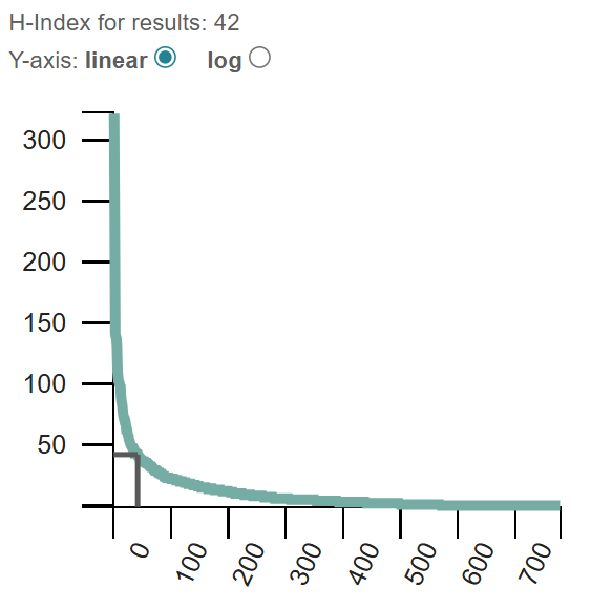
\includegraphics[width=\textwidth]{fig/fig_04_p21.png}\\[0.3em]
                {\small 引用分布（H-index = 42）}
            \end{center}
        \end{column}
        \begin{column}{0.48\textwidth}
            \begin{center}
                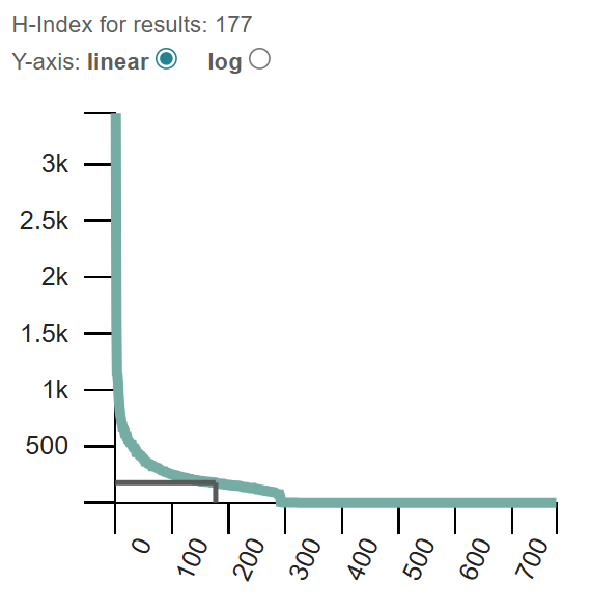
\includegraphics[width=\textwidth]{fig/fig_05_p22.png}\\[0.3em]
                {\small 阅读数据（H-index = 175）}
            \end{center}
        \end{column}
    \end{columns}
    \vspace{0.5em}
    \begin{block}{意义}
        \begin{itemize}
            \item 778篇核心文献中763篇（98.07\%）为同行评议期刊论文
            \item 总引用8393次，篇均10.79次——持续学术关注度
        \end{itemize}
    \end{block}
\end{frame}

\begin{frame}{为何射电路径长期居于主流}
    \begin{block}{物理优势}
        \begin{itemize}
            \item 射电波段的单光子能量较低，适合长距离、持续承载信息传输
            \item 射电波穿越地球大气衰减最小
            \item 星际介质对射电信号衰减相对可控
        \end{itemize}
    \end{block}

    \begin{block}{技术优势}
        \begin{itemize}
            \item 成熟的技术链条：窄带检测、多普勒漂移修正、RFI排除、重复观测
            \item 与常规射电天文设备重合度高，可"搭载式"运行
            \item 德雷克方程提供量化分析框架
        \end{itemize}
    \end{block}

    \defination{核心要点}{
        射电SETI的长盛不衰不仅是偏好，而是物理基础、技术成熟度和制度"搭载"可行性的共同支撑。
    }
\end{frame}

% ============================================================
\section{SETI与传统天文科学的范式差异}
% ============================================================

\begin{frame}{范式差异：SETI与传统天文学}
    \begin{table}
        \centering\small
        \begin{tabular}{lp{3.2cm}p{3.2cm}}
            \hline
            \textbf{比较维度} & \textbf{传统观测天文学} & \textbf{SETI} \\
            \hline
            研究对象 & 对象已知存在 & 是否存在本身不确定 \\
            零结果含义 & 可直接压缩模型参数 & 只能排除局部假设 \\
            正结果门槛 & 重复观测+模型拟合 & 须排除RFI、设备伪迹和所有自然过程 \\
            成果评价 & 精度和样本规模 & 公众易只关注"是否发现" \\
            资金制度 & 嵌入稳定观测体系 & 依赖专项倡议与附加机时 \\
            \hline
        \end{tabular}
    \end{table}

    \begin{block}{以宇宙学为参照}
        宇宙学从"思辨性过强"到"精确宇宙学"的转化，靠的不是哲学辩护，而是观测能力的进步（COBE、Planck等）。SETI需要同样的路径：把"听了很久没听到"变成清晰的参数空间约束。
    \end{block}
\end{frame}

% ============================================================
\section{SKA驱动的三维度跃升}
% ============================================================

\begin{frame}{频率维度：从局部窗口到设施级宽频覆盖}
    \begin{center}
        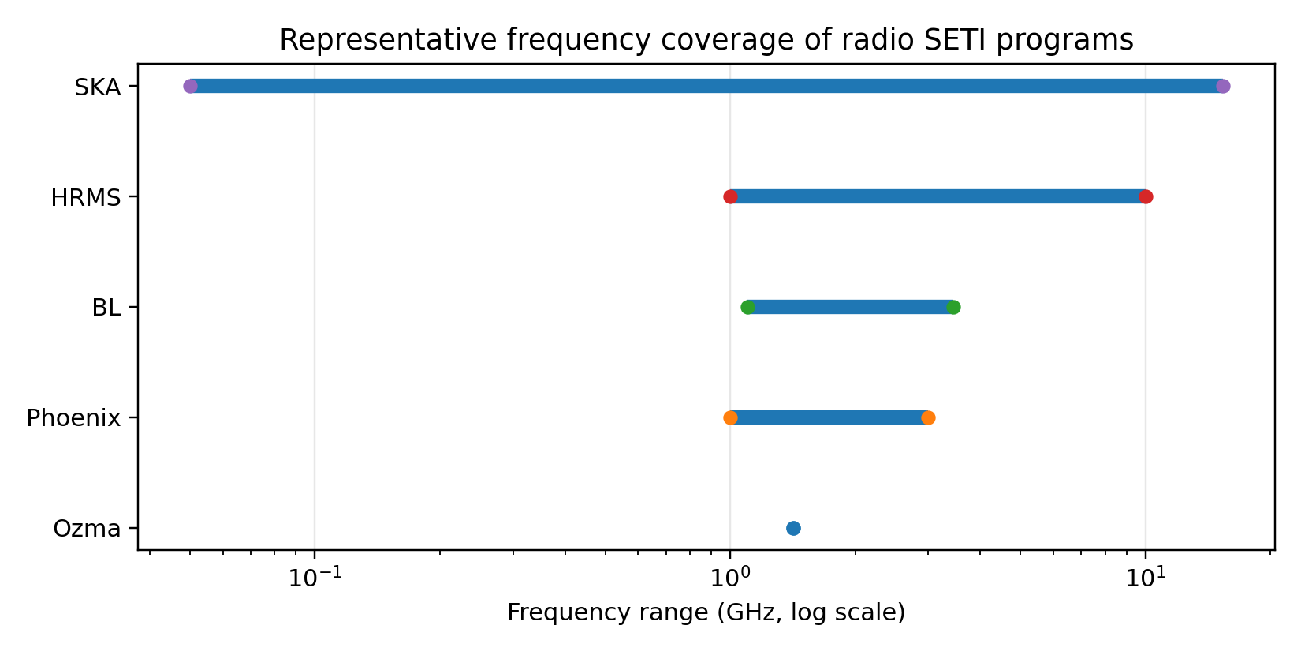
\includegraphics[width=0.75\textwidth]{fig/fig_06_p28.png}
    \end{center}
    \vspace{-0.3em}
    {\small 图5.1 代表性射电SETI计划的频率跨度比较}

    \begin{block}{数量级跃升}
        \begin{itemize}
            \item 奥兹玛：$\sim$1.42 GHz单频点；凤凰：1--3 GHz；BL：1.10--3.45 GHz
            \item SKA-Low：50--350 MHz + SKA-Mid：0.35--15.4 GHz = 设施级宽频覆盖
            \item 减少对"水洞"频段的先验偏好，系统扩展搜索频段
        \end{itemize}
    \end{block}
\end{frame}

\begin{frame}{天区维度：从点目标监听走向可累积覆盖}
    \begin{center}
        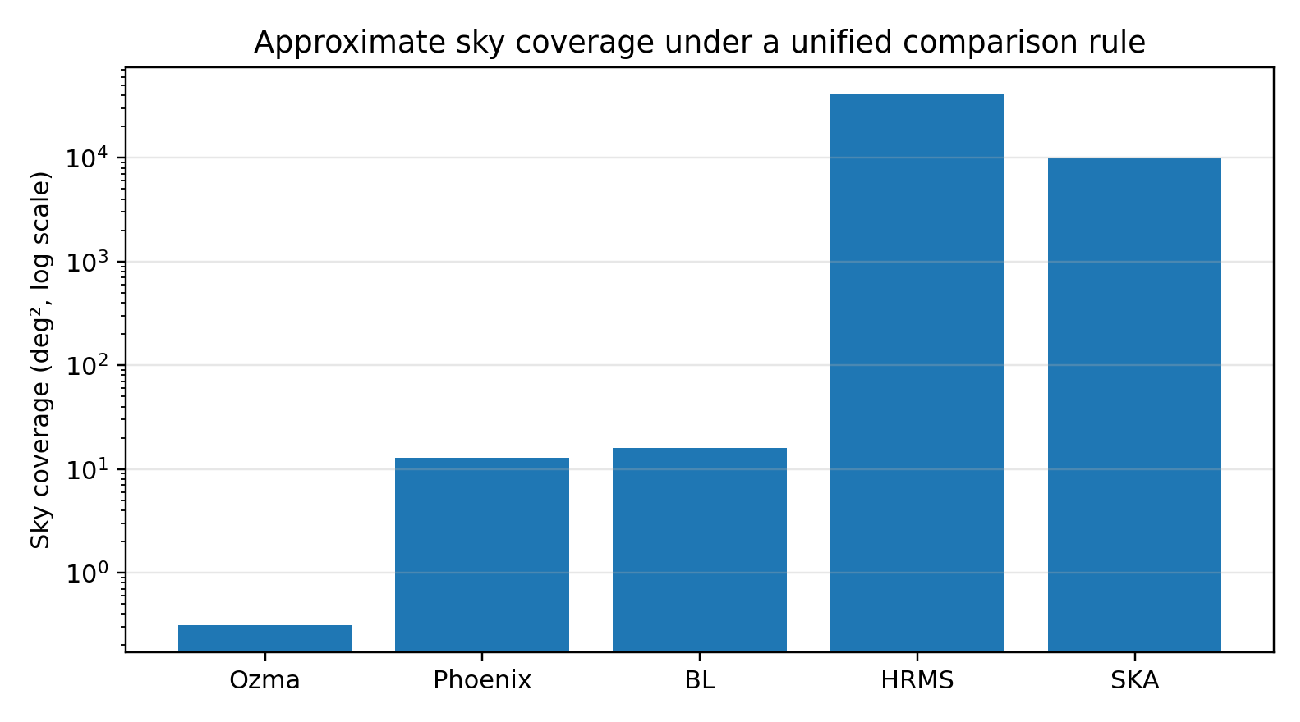
\includegraphics[width=0.75\textwidth]{fig/fig_07_p29.png}
    \end{center}
    \vspace{-0.3em}
    {\small 图5.2 代表性射电SETI计划的天区覆盖比较（对数坐标）}

    \begin{block}{搜索策略的结构升级}
        \begin{itemize}
            \item 奥兹玛：$\sim$0.31 deg$^2$；凤凰：$\sim$12.8 deg$^2$；BL：$\sim$16.0 deg$^2$
            \item SKA：预期可累积覆盖 $10^3$--$10^4$ deg$^2$（通过共享观测）
            \item 首次实现深搜与广域巡天在同一设施体系内并存
        \end{itemize}
    \end{block}
\end{frame}

\begin{frame}{灵敏度维度：SKA的价值不只是"口径更大"}
    \begin{center}
        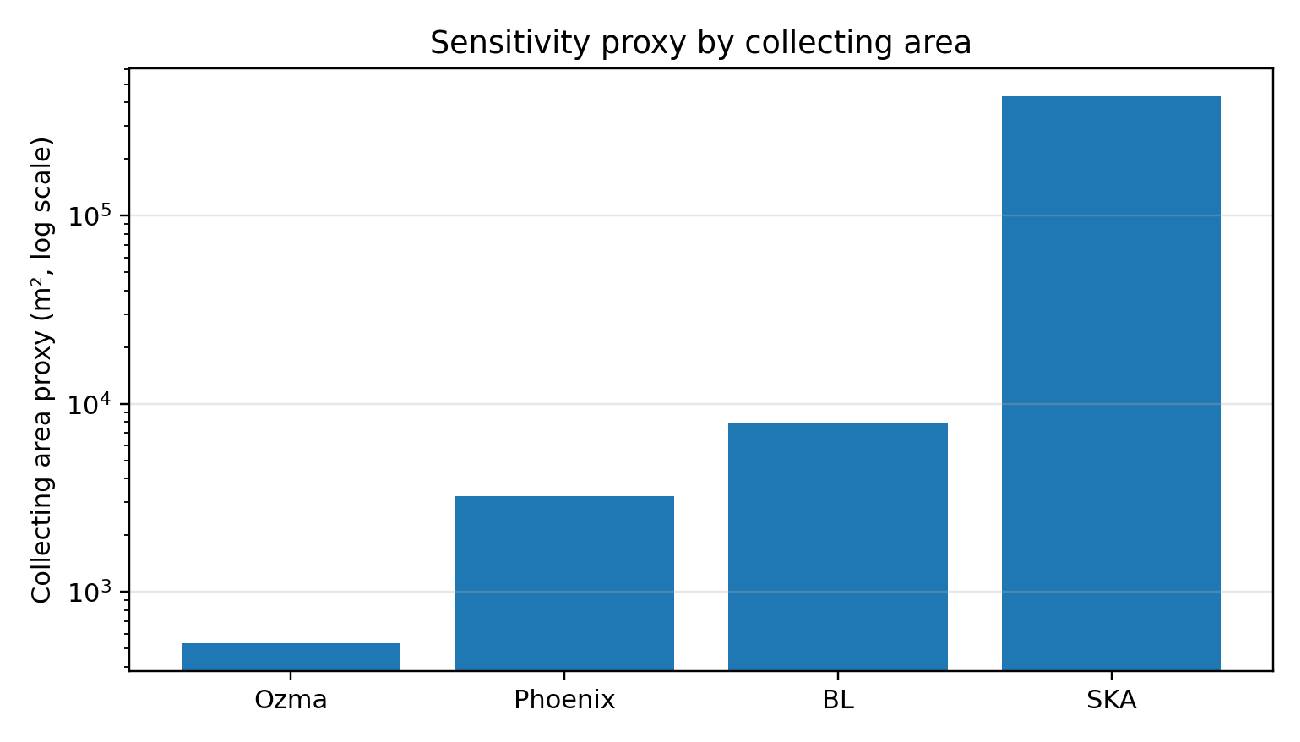
\includegraphics[width=0.75\textwidth]{fig/fig_08_p32.png}
    \end{center}
    \vspace{-0.3em}
    {\small 图5.3 以集光面积为代理的灵敏度比较（对数坐标）}

    \begin{block}{关键公式}
        \begin{itemize}
            \item 辐射计方程：$S_{\min} \approx \dfrac{(S/N)_{\min} \cdot \text{SEFD}}{\sqrt{n_p \, \Delta\nu_{\text{ch}} \, t_{\text{int}}}}$
            \item EIRP约束：$\text{EIRP}_{\min} \approx 4\pi d^2 \, S_{\min} \, \Delta\nu_{\text{sig}}$
            \item SKA1总集光面积 $\sim 4.33 \times 10^5$ m$^2$，比任何单口径高1--2个数量级
        \end{itemize}
    \end{block}
\end{frame}

\begin{frame}{三维同步扩张与"零结果"的新含义}
    \theorem{核心发现}{
        SKA有望首次实现天区覆盖、频率覆盖和灵敏度三项关键能力的\textbf{同步扩张}，使长期难以形成强约束的"零结果"转化为更明确的参数空间上界。
    }

    \begin{table}
        \centering\small
        \begin{tabular}{lccc}
            \hline
            \textbf{项目} & \textbf{天区（deg$^2$）} & \textbf{频率（GHz）} & \textbf{集光面积（m$^2$）} \\
            \hline
            奥兹玛计划 & 0.31 & 1.42（单频） & $\sim$531 \\
            凤凰计划 & 12.8 & 1--3 & $\sim$3,217 \\
            Breakthrough Listen & 16.0 & 1.10--3.45 & $\sim$7,854 \\
            NASA HRMS & $4.1 \times 10^4$ & 1--10 & 多设施 \\
            \textbf{SKA} & $\mathbf{10^3}$--$\mathbf{10^4}$ & \textbf{0.05--15.4} & $\mathbf{\sim 4.3 \times 10^5}$ \\
            \hline
        \end{tabular}
    \end{table}
\end{frame}

% ============================================================
\section{结论与展望}
% ============================================================

\begin{frame}{主要结论}
    \begin{block}{1. 文献统计发现}
        SETI的兴衰更主要受\textbf{设备能力、资助结构及相关学科发展条件}影响，而非单纯取决于是否发现可信信号。
    \end{block}

    \begin{block}{2. 三维框架价值}
        天区覆盖 $\times$ 频率覆盖 $\times$ 灵敏度的三维框架，可有效揭示历史计划与SKA之间的\textbf{结构性差异}。
    \end{block}

    \begin{block}{3. SKA核心意义}
        SKA对SETI的核心意义不在于保证发现地外文明，而在于\textbf{重塑其证据基础与成果评价方式}，推动SETI走向以参数空间约束为特征的观测科学。
    \end{block}

    \begin{block}{4. 范式转化}
        首次实现三项关键能力的同步扩张，使零结果从弱约束转化为参数空间的\textbf{明确上界}。
    \end{block}
\end{frame}

\begin{frame}{对SETI发展的思考与展望}
    \begin{block}{共享观测优先}
        SETI后端可与常规天文观测并行运行，无需单独占用望远镜时间，最大化观测效率。
    \end{block}

    \begin{block}{多波段联动}
        射电仍应作为主轴，但光学、红外、紫外等多波段联动可提供技术特征搜索的交叉验证。
    \end{block}

    \begin{block}{算法方法支撑}
        机器学习与信号处理算法在RFI排除、候选目标筛查与复核中发挥关键作用。
    \end{block}

    \begin{block}{零结果正式化}
        将零结果当作正式科学产出，建立规范化的参数空间约束报告体系。
    \end{block}

    \begin{block}{与系外行星和天体生物学协同}
        结合系外行星和宜居性研究，为technosignature搜索提供更扎实的科学语境。
    \end{block}
\end{frame}

% ============================================================
\section{致谢}
% ============================================================

\begin{frame}
    \begin{center}
        {\Huge\textbf{感谢各位专家评委的指导！}}\\[2em]
        {\Large 谢谢！}\\[1em]
        {\normalsize 答辩人：王伊煜 \quad|\quad 22344140}\\[0.3em]
        {\small 指导教师：张泳 教授\\
        中山大学 物理与天文学院}
    \end{center}
\end{frame}

\end{document}
